\begin{frame}
\frametitle{About This Work...}

\emph{Probabilistic Threshold $k$ Nearest Neighbor Queries over Moving Objects in Symbolic Indoor Space}.~\cite{DBLP:conf/edbt/YangLJ10} \\
B.~Yang, H.~Lu, and C.~S. Jensen.\\~\\

\begin{itemize}
  \item Published in year 2010 at the \emph{EDBT} conference.
  \item \emph{Minimal Indoor Walking Distance}(MIWD) along with algorithms and data structures are proposed for distance computing and storage.
  \item Effective object indexing structures, also capture the uncertainty of object locations.
  \item On this foundation, Probabilistic threshold $k$NN (PT$k$NN) query is studied.
\end{itemize}

\end{frame}
%------------------------------------------------

\begin{frame}
\frametitle{Motivation}

\begin{itemize}
  \item Indoor positioning makes it possible to support interesting queries over large populations of moving objects.
    \begin{itemize}
      \item shopping mall, airports, office buildings
      \item $k$NN queries over indoor moving objects enables the detection of approaching potential threats at sensitive locations in a subway system
    \end{itemize}

  \item Existing $k$NN techniques in spatial and spatialtemporal databases are inapplicable in indoor spaces.
    \begin{itemize}
      \item complex entities and topologies
      \item indoor positioning techniques differ fundamentally from outdoor GPS, low sampling frequency and accuracy
    \end{itemize}
\end{itemize}

\end{frame}
%------------------------------------------------

\begin{frame}
\frametitle{Minimal Indoor Walking Distance}

\emph{Minimal Indoor Walking Distance}(MIWD) is used as the distance metric in indoor spaces.
\pause

The mapping $\mathnormal{Rooms}$ determines the room of an indoor position:
\pause
\begin{equation}
\mathnormal{Rooms: positions \rightarrow \Sigma_{rooms}}
\end{equation}

\pause

The mapping $\mathnormal{Doors}$ maps a room to the doors that connect the room to an adjacent room:
\pause
\begin{equation}
\mathnormal{Doors: \Sigma_{rooms} \rightarrow 2^{\Sigma_{doors}}}
\end{equation}

\end{frame}

%------------------------------------------------

\begin{frame}
\frametitle{Minimal Indoor Walking Distance}

\begin{columns}[c]
  \column{.52\textwidth}
  \begin{figure}[tb]
    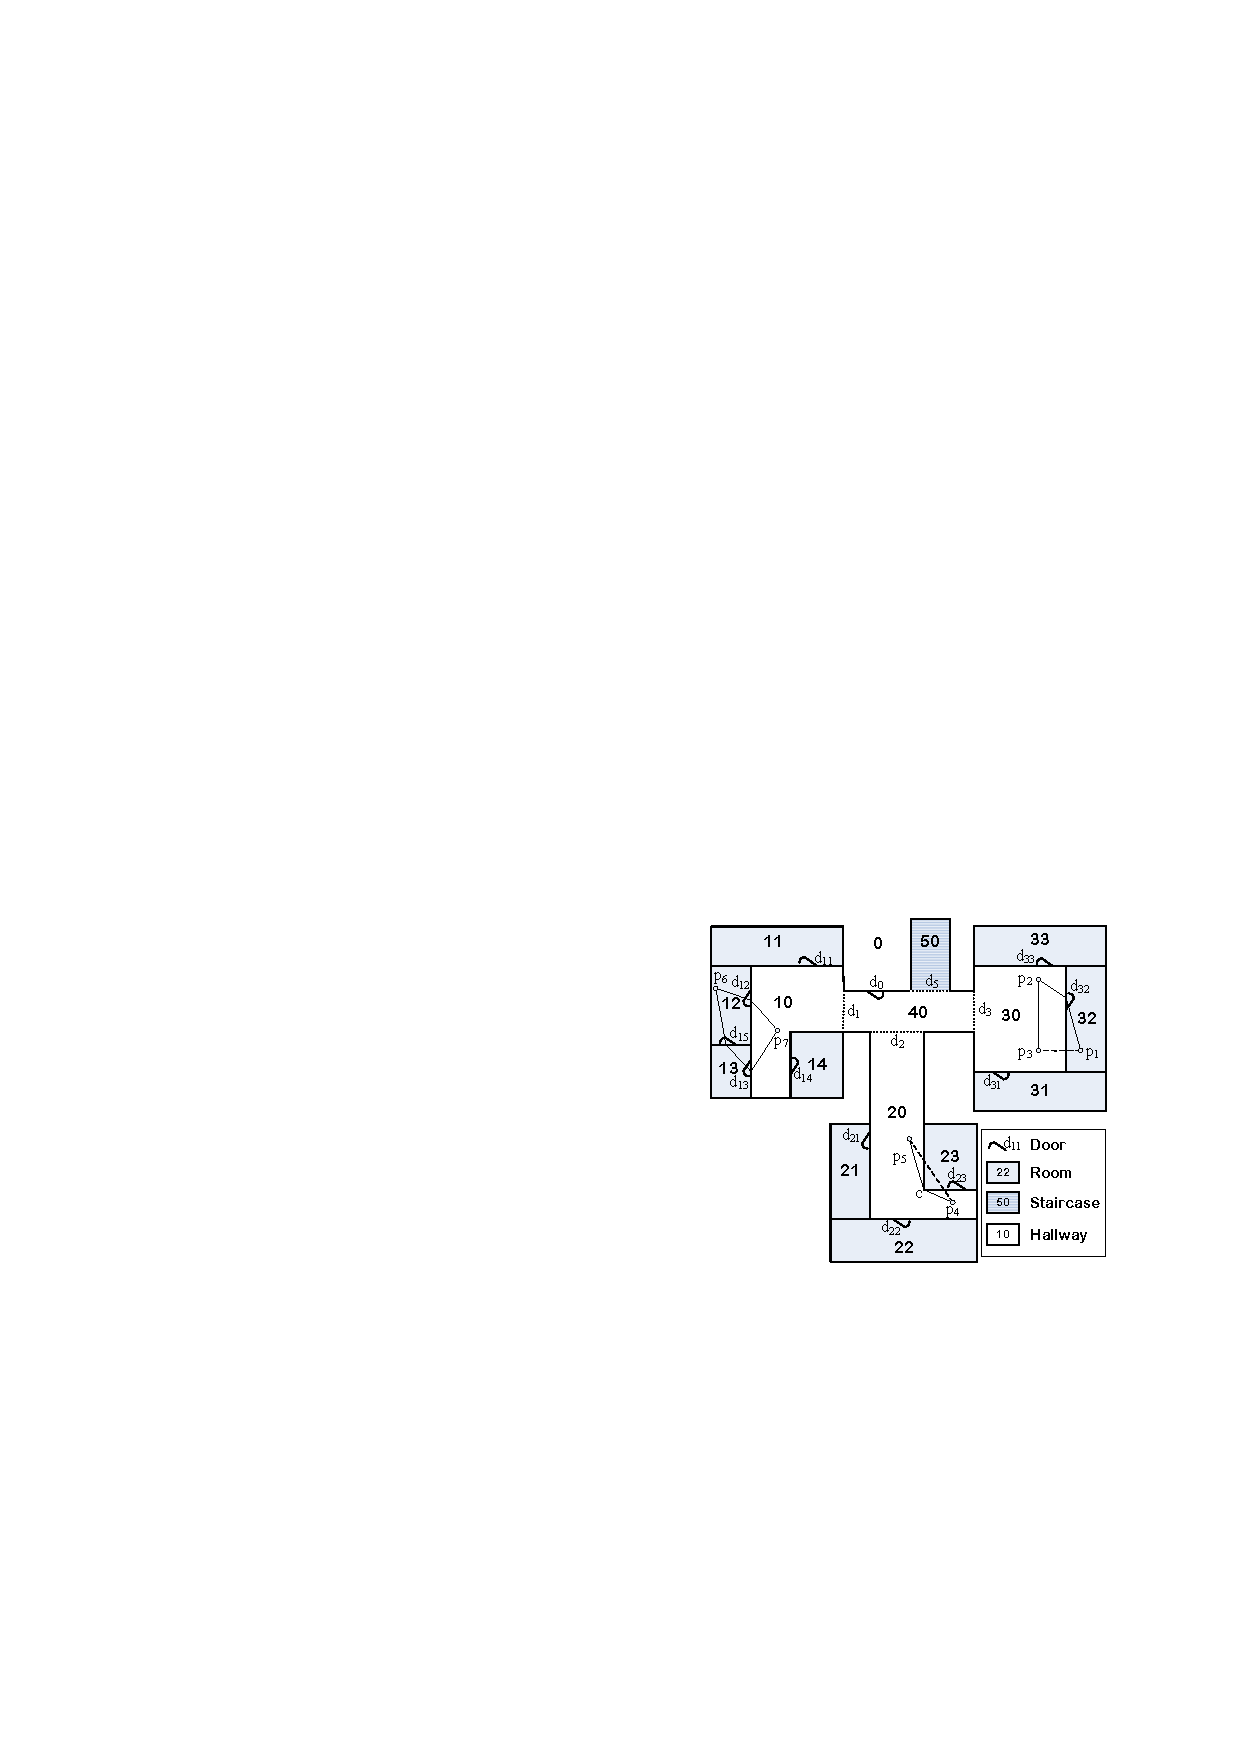
\includegraphics[width=\columnwidth]{figures/2-3/2-3-1.pdf}
  \end{figure}

  \column{.48\textwidth}
  \begin{itemize}
    \scriptsize{
    \item intra-room obstructed distance, termed as $\mathnormal{d_o}$. E.g., $\mathnormal{d_o(p_2, p_3) = |p_2p_3|}$ and $\mathnormal{d_o(p_4, p_5) = |p_4c|+|cp_5|}$.
    \item if in different rooms, it should take into account the doors connecting the rooms. E.g., $\mathnormal{d_{MIN}(p_1, p_2) = |p_1d_{32}| + |d_{17}p_9|}$.
    \item if there exist several paths, the correct path should be the shortest one. E.g., $\mathnormal{d_{MIN}(p_6, p_7) = |p_6d_{12}| + |d_{12}p_7|}$ $\mathnormal{\neq |p_6d_{15}| + |d_{15}d_{13}| + |d_{13}p_7|}$.
    }
  \end{itemize}

\end{columns}

\end{frame}

%------------------------------------------------

\begin{frame}
\frametitle{Minimal Indoor Walking Distance}

\emph{Doors Graph} is capable of retrieving the connecting doors between two rooms, which is convenient for computing MIWD.

\begin{columns}[c]

  \column{.48\textwidth}
    \begin{figure}[tb]
      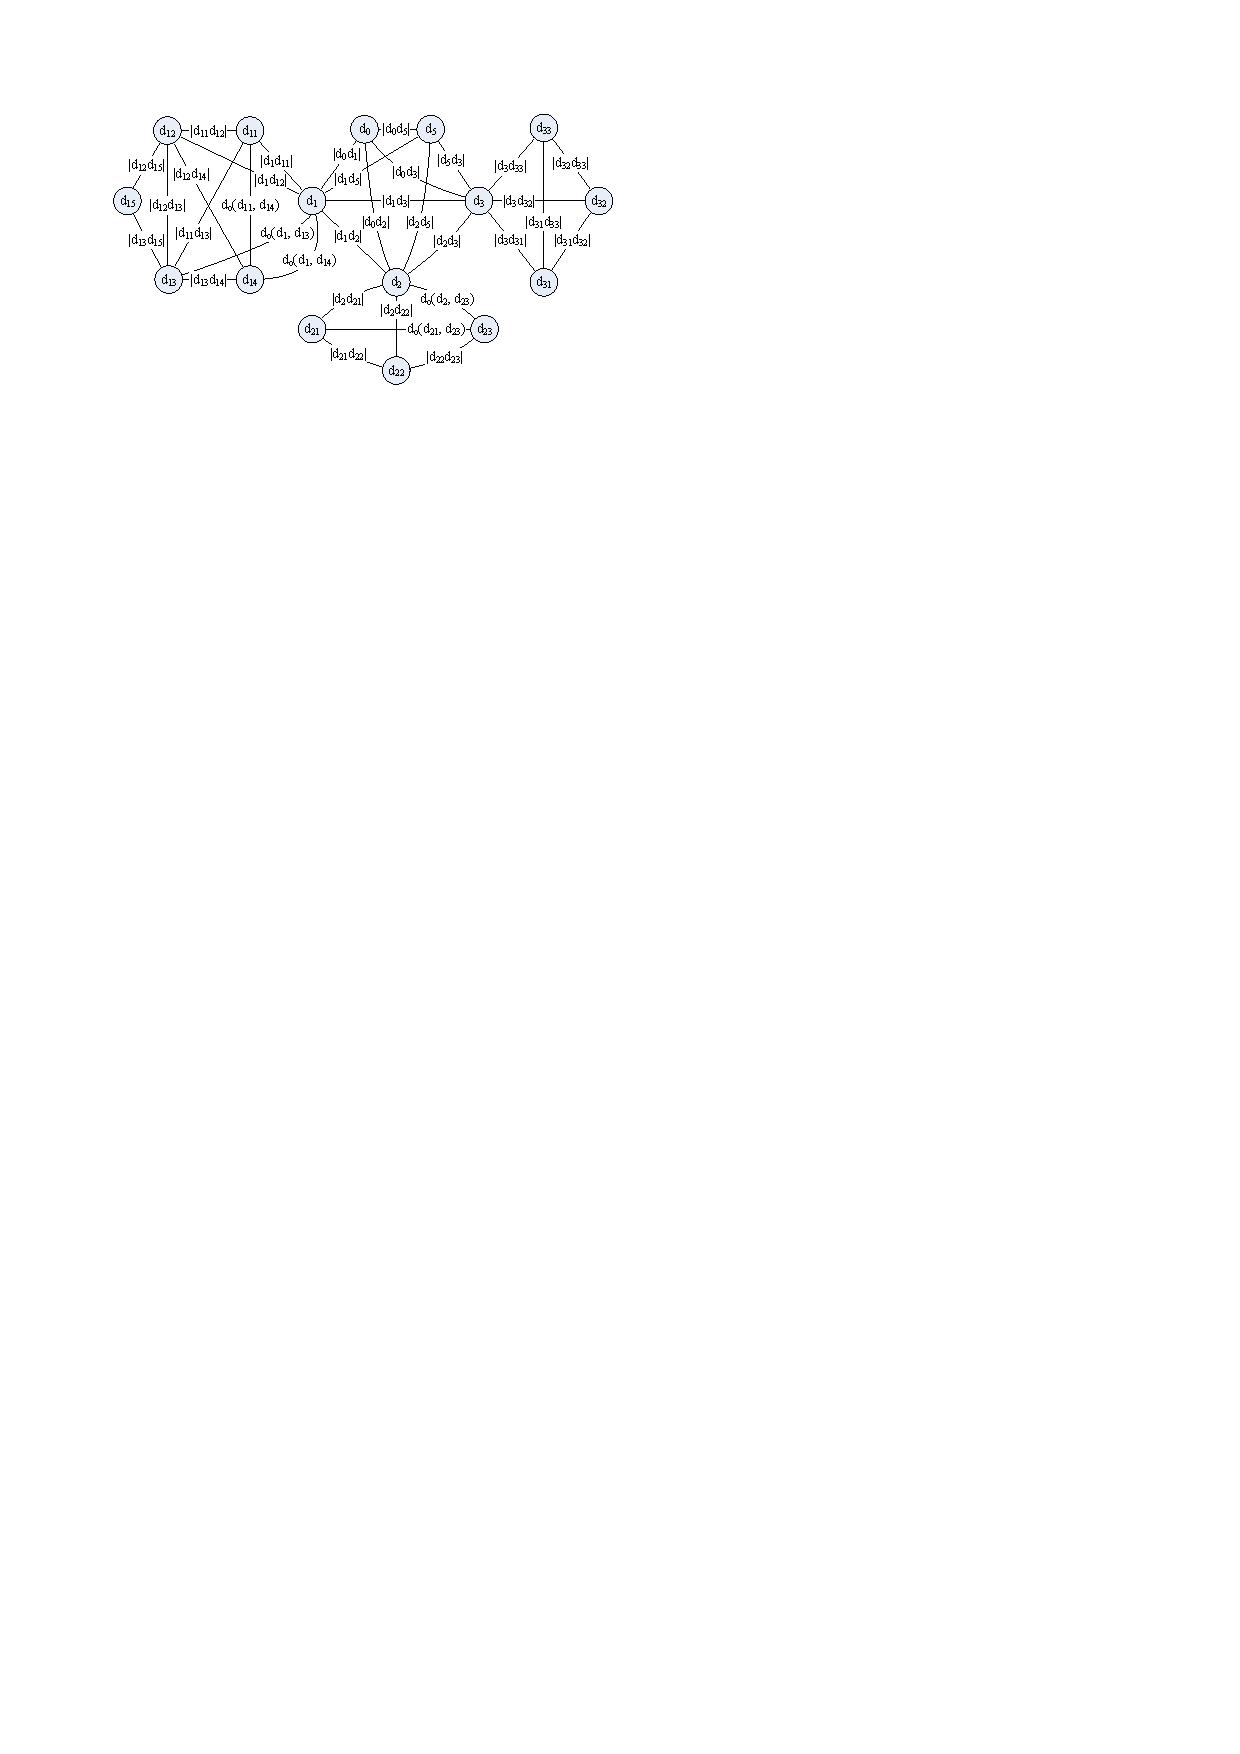
\includegraphics[width=\columnwidth]{figures/2-3/2-3-2.pdf}
    \end{figure}

  \column{.52\textwidth}
    \begin{block}{Doors Graph}
      \textrm{
      \footnotesize{
      \begin{itemize}
        \item $\mathnormal{G_{d} = \{ D, E, l_{weight} \}}$
        \item $\mathnormal{D = \Sigma_{doors}}$ is the set of the vertices
        \item $\mathnormal{E}$: An edge $\mathnormal{\{ d_i, d_j \}}$ exists if a room $\mathnormal{rm}$ exists in $\mathnormal{\Sigma_{rooms}}$ such that $\mathnormal{\{ d_i, d_j \} \subseteq Doors(rm)}$
        \item $\mathnormal{l_{weight}: E \rightarrow R}$ assigns to an edge the obstructed distance between the two doors as $\mathnormal{d_o(d_i, d_j)}$
      \end{itemize}
      }
      }
    \end{block}

\end{columns}

\end{frame}

%------------------------------------------------

\begin{frame}
\frametitle{Minimal Indoor Walking Distance}

All door-to-door shortest path distances can be computed and recorded in a hash table $\mathrm{D2D}$ according to the Doors Graph.
\pause
\begin{equation}
  \mathrm{D2D}: \mathnormal{ \{ (d_p, d_j) \} \rightarrow R, ~~d_p, d_q \in \Sigma_{doors} }.
\end{equation}
\pause
Consequently, for two positions $\mathnormal{p}$ and $\mathnormal{q}$ in different rooms.
\pause
\begin{equation}
  \mathnormal{d_{MIN}(d_p, d_q) = d_o(p, d_p) + \mathrm{D2D}(d_p, d_q) + d_o(d_q, q)}
\end{equation}
where $\mathnormal{d_p(d_q)}$ ranges over all doors of room $\mathnormal{p(q)}$.

\begin{columns}[c]

  \column{.48\textwidth}
    \begin{figure}[tb]
      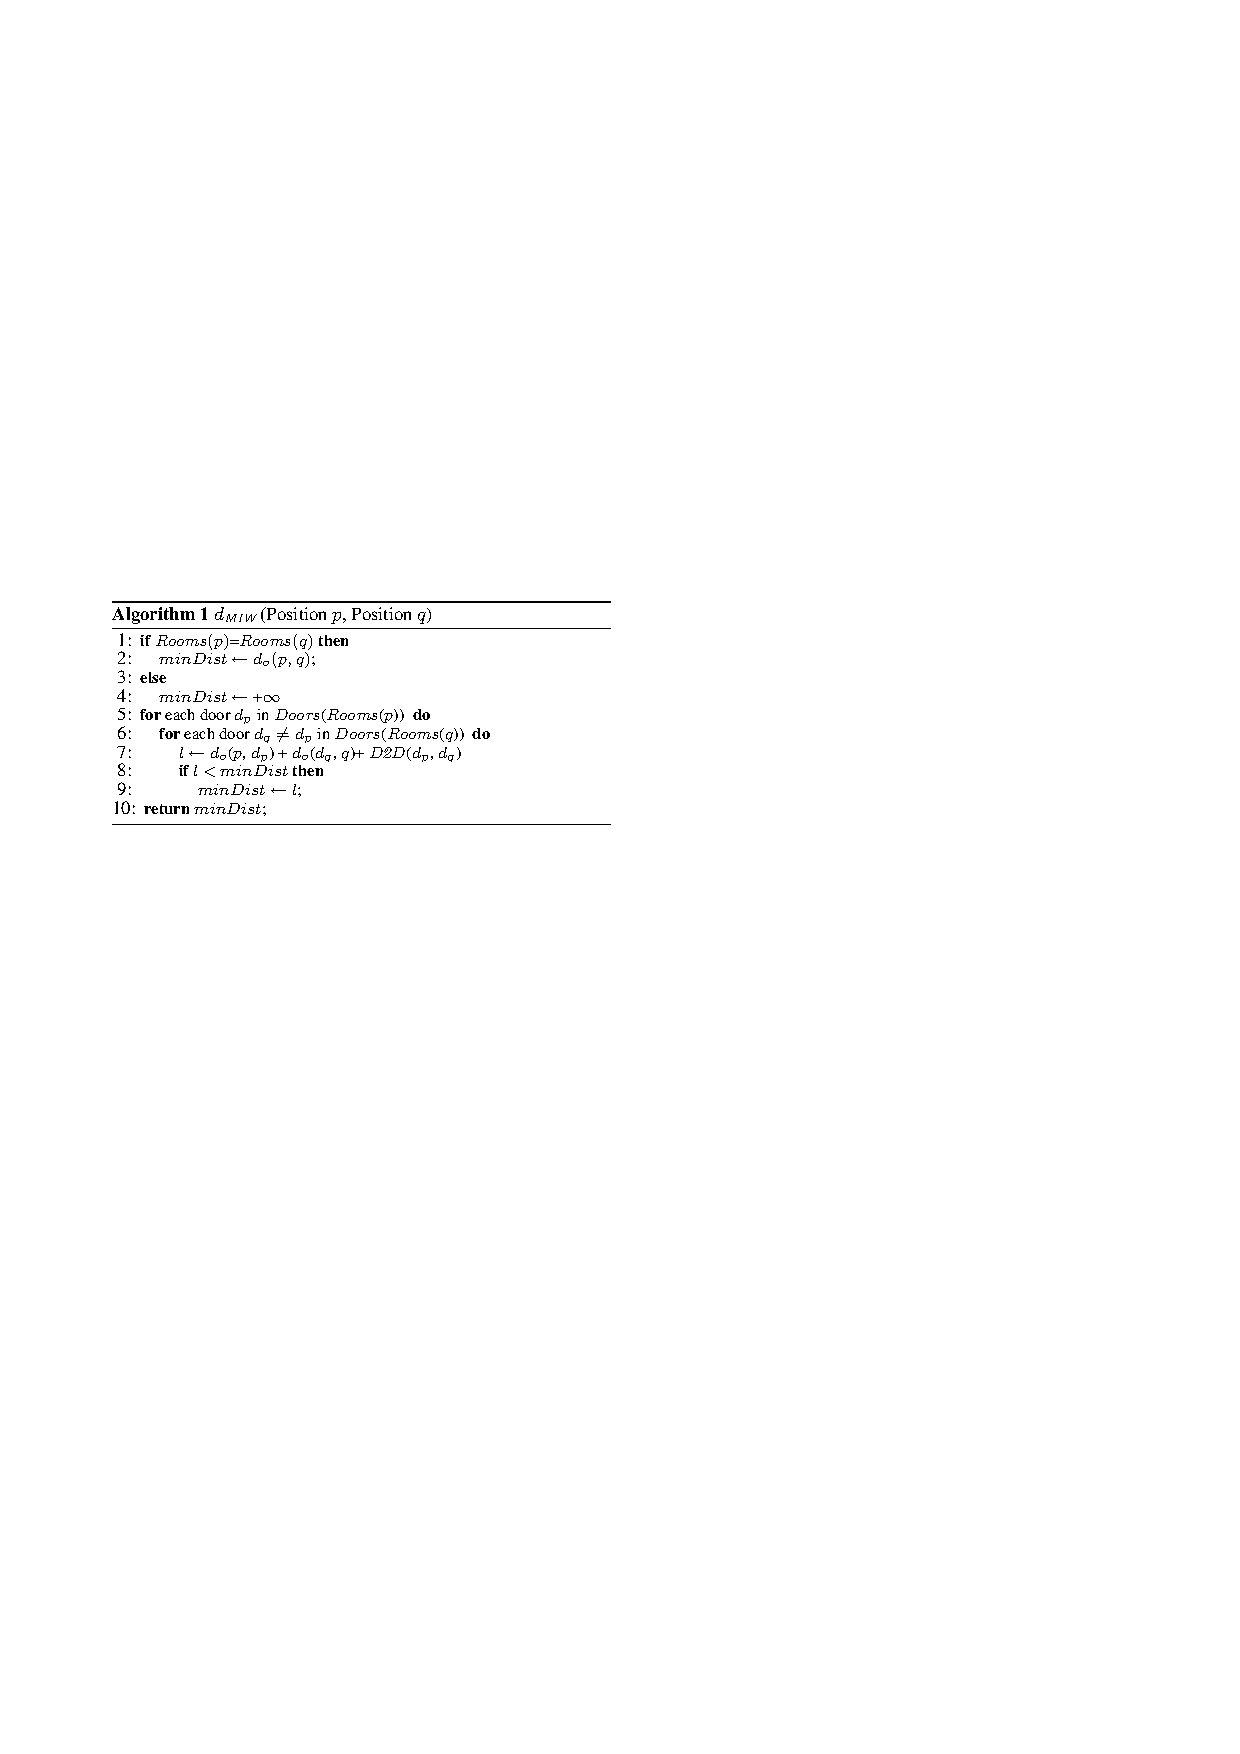
\includegraphics[width=\columnwidth]{figures/2-3/2-3-3.pdf}
    \end{figure}

  \column{.52\textwidth}
    \scriptsize{
    it is possible to adapt this notion of distance to accommodate other semantics. For example, a person might prefer a longer indoor path that passes as few doos as possible.
    }
    
\end{columns}

\end{frame}
